\documentclass{scrbook}
\usepackage{graphicx} % Required for inserting images
\usepackage{tabularx} % Required for fixed width tables
\usepackage{scrlayer-scrpage} % Required for the subtitles
\usepackage{url} % Required for the URLs
\usepackage{hyperref} % Required for the URLs
\usepackage{listings} % Required for the code snippets
\usepackage{mathtools} % Required for the system of equations
\usepackage{enumitem} % Required for list styling

\usepackage{fontspec}
\setmonofont{DejaVu Sans Mono} % Overleaf has this font pre-installed

% Put the caption of the snippets at the bottom
\lstset{
	captionpos=b,
	basicstyle=\ttfamily\small,
	columns=fullflexible,
	keepspaces=true
}


\title{PHP: Hypertext Preprocessor}
\subtitle{Ambient intelligence course (A.Y. 2025/2026)\\Topic taught by Prof. Floriano Scioscia}
\author{Gabriele Colapinto}
\date{\today}

\begin{document}
	
	\maketitle
	\thispagestyle{empty}
	
	{\Large\textbf{License}} \\
	{Notes from Ambient intelligence (A.Y. 2025/2026) by Gabriele Colapinto. 
		Course taught by professors Michele Ruta, Floriano Scioscia, Arnaldo Tomasino, Davide Loconte — 
		Licensed under CC BY-NC 4.0.\\
		\url{https://creativecommons.org/licenses/by-nc/4.0/}}
	
	\vspace*{\fill}
	\rule{\textwidth}{0.2pt}
	\small{© 2025 Gabriele Colapinto \\
		Released under the \href{https://creativecommons.org/licenses/by-nc/4.0/}{Creative Commons Attribution–NonCommercial 4.0 International License}}
	
	\clearpage
	
	\tableofcontents
	
	\chapter{Introduction to PHP and Server-Side Execution}
	
	\section{Purpose and Execution Model}
	
	PHP, recursively expanded as \emph{PHP: Hypertext Preprocessor}, is a server-side scripting language used to generate dynamic Web content. In a PHP-based application, the browser does not execute the PHP program. The browser sends an HTTP request to the Web server; the server reads the requested \texttt{.php} file, interprets the PHP fragments, and returns the generated result as plain HTML to the client.\\
	
	A PHP file may contain ordinary HTML, CSS, and JavaScript, interleaved with PHP code. The static parts are copied into the response, while the PHP scripts are executed on the server. Their output is inserted at the corresponding position in the generated page. This is the essential difference between the PHP source file and the HTML document finally received by the browser: the client observes the result of the computation, not the PHP code that produced it.\\
	
	This execution model makes PHP suitable for pages whose content depends on application state, user input, database content, session data, configuration parameters, or other server-side resources. In typical use, PHP generates the dynamic portions of an otherwise HTML-based page.
	
	\section{Historical Development}
	
	PHP originated in 1995, when Rasmus Lerdorf wrote several Common Gateway Interface programs in C to maintain his personal homepage. These personal tools evolved into a server-side scripting language for dynamic Web pages.\\
	
	The development of PHP can be summarized through the following milestones:
	
	\begin{itemize}
		\item \textbf{1995}: PHP 1.0, originally called \emph{Personal Home Page Tools} (PHP Tools).
		\item \textbf{1997}: PHP 2.0, also known as \emph{PHP/FI 2.0}, became the first standalone release of the language.
		\item \textbf{1998}: PHP 3.0 was based on a substantial rewrite by Zeev Suraski and Andi Gutmans; from this version the recursive acronym \emph{PHP: Hypertext Preprocessor} became established.
		\item \textbf{2000}: PHP 4.0 introduced the Zend Engine as the parse-and-execute infrastructure for PHP scripts.
		\item \textbf{2001}: PHP 4.1 added superglobal variables such as \texttt{\$\_GET}, \texttt{\$\_POST}, and \texttt{\$\_SESSION}.
		\item \textbf{2002}: PHP 4.3 introduced the command-line interface.
		\item \textbf{2004}: PHP 5.0 introduced Zend Engine II and a new object model.
		\item \textbf{2006}: PHP 5.2 added native JSON support.
		\item \textbf{2013}: PHP 5.5 introduced \texttt{finally} blocks for exception handling.
		\item \textbf{2014}: PHP 5.6 added several language improvements.
		\item \textbf{N/A}: PHP 6.x was not released.
		\item \textbf{2015}: PHP 7.0 introduced Zend Engine 3 and important performance improvements.
		\item \textbf{2016}: PHP 7.1 added features such as \texttt{void} return type declarations, class constant visibility modifiers, and nullable types.
		\item \textbf{2020}: PHP 8.0 introduced Just-In-Time compilation, the \texttt{match} expression, attributes, and the \texttt{mixed} type.
		\item \textbf{PHP 8.x}: later PHP 8 releases continued the evolution with enumerations, readonly properties and classes, and fibers.
	\end{itemize}
	
	For this course, the important point is not the complete language history, but the progressive evolution from a simple templating and scripting tool toward a full programming language with structured server-side execution, database integration, and object-oriented features.
	
	\section{Development Environment}
	
	A PHP development setup requires the following components:
	
	\begin{itemize}
		\item a PHP distribution, providing the interpreter and standard runtime;
		\item a Web server, commonly Apache or nginx;
		\item a text editor or integrated development environment, such as Eclipse, NetBeans, or PhpStorm;
		\item a Web browser for testing the generated pages;
		\item optionally, a DBMS when the application stores or retrieves persistent data.
	\end{itemize}
	
	These components are often distributed together in all-in-one development environments such as XAMPP, WAMP, and AMPPS. They simplify local setup by providing a preconfigured stack including the Web server, PHP, and often a database system.\\
	
	The course also mentions WAPPStack as a complete integrated stack for PHP development. Its basic package includes PHP, PostgreSQL, and Apache, while additional packages may include FastCGI, OpenSSL, phpPgAdmin, ModSecurity, SQLite, and related tools. Such packaged stacks are useful for development and preliminary testing, but production deployments require explicit configuration choices, especially for security, permissions, network exposure, and database credentials.
	
	\section{Basic PHP Syntax}
	
	PHP source files conventionally use the \texttt{.php} extension. A PHP file can contain ordinary HTML markup together with PHP script blocks. PHP code may appear anywhere in the document where server-side computation is needed. A script block starts with \texttt{\textless?php} and ends with \texttt{?\textgreater}. The following example shows the basic delimiters and comment styles:
	
	\begin{lstlisting}
	<?php
	  // PHP code goes here (single-line comment)
		
	  # This is also a single-line comment
		
	  /*
		This is a multi-line comment block
		that spans over multiple lines.
	  */
	?>
	\end{lstlisting}
	
	The delimiters are significant because they separate server-side instructions from the static content that will be sent directly to the client. Code outside PHP delimiters is not interpreted as PHP; it is treated as part of the output document.
	
	\section{A First PHP Page}
	
	The following file, conventionally named \texttt{HelloWorld.php}, contains an HTML page with one PHP instruction embedded in the body. The \texttt{echo} instruction writes text into the server-generated output stream.
	
	\begin{lstlisting}
	<!DOCTYPE html>
	<html>
	  <body>
		
		<h1>My first PHP page</h1>
		
		<?php
		  echo "Hello World!";
		?>
		
	  </body>
	</html>
	\end{lstlisting}
	
	When the file is requested through the Web server, the PHP interpreter executes only the PHP block. The generated document sent to the browser is plain HTML:
	
	\begin{lstlisting}
	<!DOCTYPE html>
	<html>
	  <body>
		
		<h1>My first PHP page</h1>
		
		Hello World!
		
	  </body>
	</html>
	\end{lstlisting}
	
	\begin{figure}
		\centering
		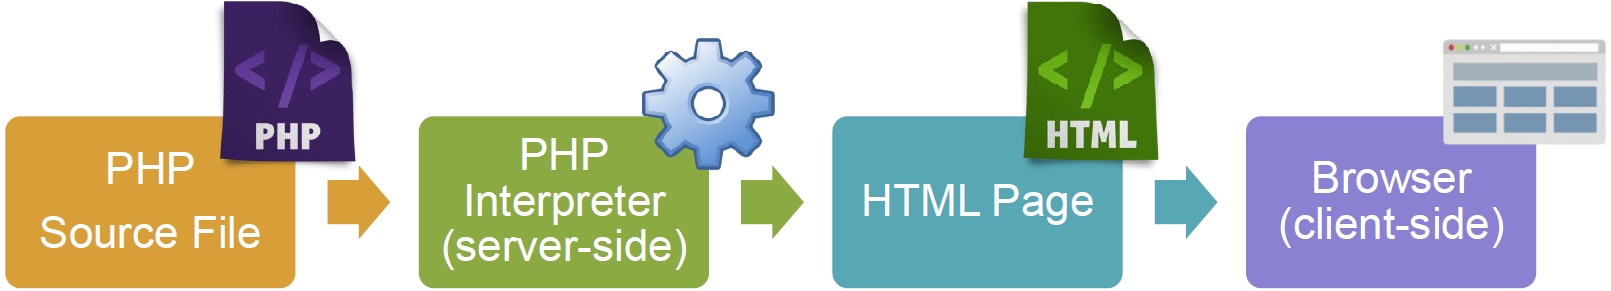
\includegraphics[width=\linewidth]{Images/PHP_to_HTML.png}
		\caption{Workflow that turns a PHP document into an HTML page and delivers it to the client}
		\label{fig:php_to_html}
	\end{figure}
	
	The resulting workflow is therefore (see figure \ref{fig:php_to_html}):
	
	\begin{itemize}
		\item the client requests the PHP source file from the server;
		\item the PHP interpreter executes the server-side script blocks;
		\item the dynamic output is inserted into the HTML response;
		\item the browser receives and renders the generated HTML page.
	\end{itemize}
	
	The browser never receives the original PHP instruction. It receives only the output produced by that instruction, together with the static HTML surrounding it.
	
	\chapter{Core PHP Language Elements}
	
	\section{Variables and Dynamic Typing}
	
	PHP variables are identified by a leading dollar sign followed by the variable name. The name must begin with a letter or an underscore, may contain letters, digits, and underscores, and is case-sensitive: \texttt{\$age} and \texttt{\$AGE} denote different variables. A variable is created when a value is first assigned to it; there is no separate declaration step for ordinary variables.\\
	
	PHP is loosely typed: the type associated with a variable is determined by the value currently assigned to it, and the same variable may hold values of different types during the execution of a script. The basic categories used in the slides are:
	\begin{itemize}
		\item Strings
		\item Integers
		\item Floating-point numbers
		\item Booleans
		\item Arrays
		\item Objects
		\item NULL
		\item Resources (special variables holding references to external resources)
	\end{itemize}
	
	PHP 8.0 introduces the \texttt{mixed} type for the variables that can be any of the latter listed types. It is, in type theory parlance, the top type. Meaning every other type is a subtype of it. It's the same concept as the \texttt{Any} type of Python.\\
	
	Type-checking functions such as \texttt{is\_int()}, \texttt{is\_string()}, \texttt{is\_array()}, and analogous \texttt{is\_type} predicates are available when the program must inspect the runtime type of a value.
	
	\begin{lstlisting}
	<?php
	  $txt = "Hello world!";  // string
	  $x = 5;                 // integer
	  $y = 10.5;              // float
		
	  $x = true;              // the same variable now holds a boolean value
		
	  if (is_bool($x)) {
		echo "x is boolean";
	  }
	?>
	\end{lstlisting}
	
	This flexibility is useful in small scripts and dynamic page generation, but it also increases the importance of explicit validation at the application boundary. In larger code bases, optional type declarations on function parameters, return values, and properties are typically used to make the intended data contracts explicit.
	
	\section{Variable Scope}
	
	PHP distinguishes between global, local, and static variables.
	\begin{itemize}
		\item A global variable is defined outside functions in the script scope;
		\item A local variable is defined inside a function and is normally accessible only in that function;
		\item A static local variable is also local to a function, but its value is preserved across repeated calls.
	\end{itemize}
	
	Access to a global variable from inside a function is not implicit. The function must either declare the variable with the \texttt{global} keyword or access it through the \texttt{\$GLOBALS} superglobal array. The array form treats the name of the global variable, without the dollar sign, as the key of an associative array.
	
	\begin{lstlisting}
	<?php
	  $x = 5;     // global variable
	  $y = 10;    // global variable
	
	  function myFunction() {
		// binds the global variable $y
		global $y;
		$y++;
		
		// direct update through the superglobal array
		$GLOBALS['x']++;
		
		// local variable
		$loc = 0;
		
		// local variable whose value persists across calls
		static $z = 20;
		$z++;
		
		echo "x = {$GLOBALS['x']}, y = $y, z = $z, loc = $loc\n";
	  }
	
	  myFunction(); // x = 6, y = 11, z = 21, loc = 0
	  myFunction(); // x = 7, y = 12, z = 22, loc = 0
	?>
	\end{lstlisting}
	
	Static variables are useful when a function must retain internal state without exposing that state as a global variable. They should still be used deliberately: hidden state makes reasoning about repeated calls and tests more difficult.
	
	\section{Arrays}
	
	PHP arrays cover three use cases introduced in the slides: indexed arrays, associative arrays, and multidimensional arrays.
	\begin{itemize}
		\item Indexed arrays use numeric positions, starting from zero;
		\item Associative arrays use named keys;
		\item Multidimensional arrays are arrays whose elements are themselves arrays.
	\end{itemize}
	
	\begin{lstlisting}
	<?php
	  $cars = array("Volvo", "BMW", "Toyota");
		
	  $cars[0] = "Volvo";
	  $cars[1] = "BMW";
	  $cars[2] = "Toyota";
		
	  // key => value
	  $age = array(
	 	"Peter" => "35",
		"Ben" => "37",
		"Joe" => "43"
	  );
		
	  $age['Peter'] = "35";
	  $age['Ben'] = "37";
	  $age['Joe'] = "43";
		
	  $matrix = array(
		array(1, 2, 3),
		array(4, 5, 6)
	  );
	  
	  var_dump($cars); // Prints one array
	  echo $cars[1]."\n"; // BMW
	  
	  var_dump($matrix); // Prints an array containing two arrays
	  echo $matrix[1][1]; // 5
	?>
	\end{lstlisting}
	
	The same syntactic mechanism is used for many PHP runtime structures, including superglobals. This is why form fields, request metadata, cookies, and session variables are usually accessed through associative-array notation.
	
	\section{Superglobals}
	
	Superglobals are predefined variables available in every scope of a PHP script. They are central in server-side Web programming because they expose request data, server metadata, file uploads, cookies, sessions, and environment variables.
	
	\begin{description}
		\item[\texttt{\$GLOBALS}] Associative array containing global variables, indexed by their names.
		
		\item[\texttt{\$\_SERVER}] Information about headers, paths, script locations, the Web server, and the current request.
		
		\item[\texttt{\$\_REQUEST}] Request data, commonly including submitted form data according to the server configuration.
		
		\item[\texttt{\$\_POST}] Submitted form data when the form uses \texttt{method="post"}.
		
		\item[\texttt{\$\_GET}] Submitted form data and query parameters when the request uses \texttt{method="get"} or a query string.
		
		\item[\texttt{\$\_FILES}] Files uploaded via the HTTP POST method.
		
		\item[\texttt{\$\_ENV}] Variables passed through the environment.
		
		\item[\texttt{\$\_COOKIE}] Values received from HTTP cookies.
		
		\item[\texttt{\$\_SESSION}] Session variables available to the current script after session handling has been started.
	\end{description}
	
	Because these variables may contain data supplied by the client or by the execution environment, they should not be treated as trusted application data. Their values are entry points to the application logic and must be validated before use in security-sensitive contexts.
	
	\subsection{\texttt{\$\_SERVER}}
	
	The \texttt{\$\_SERVER} array gives access to metadata about the executing script, the Web server, and the current HTTP request. The slide deck highlights the following entries:
	
	\begin{itemize}
		\item \texttt{\$\_SERVER['PHP\_SELF']}: filename of the currently executing script.
		
		\item \texttt{\$\_SERVER['SERVER\_ADDR']}: IP address of the host server.
		
		\item \texttt{\$\_SERVER['SERVER\_NAME']}: name of the host server.
		
		\item \texttt{\$\_SERVER['SERVER\_SOFTWARE']}: server identification string, for example an Apache version string.
		
		\item \texttt{\$\_SERVER['SERVER\_PROTOCOL']}: name and revision of the information protocol, for example \texttt{HTTP/1.1}.
		
		\item \texttt{\$\_SERVER['REQUEST\_METHOD']}: HTTP method used to access the page, such as \texttt{POST}.
		
		\item \texttt{\$\_SERVER['REQUEST\_TIME']}: timestamp corresponding to the start of the request.
		
		\item \texttt{\$\_SERVER['QUERY\_STRING']}: query string used to access the page, if present.
		
		\item \texttt{\$\_SERVER['HTTP\_ACCEPT']}: \texttt{Accept} header of the current request.
		
		\item \texttt{\$\_SERVER['HTTP\_HOST']}: \texttt{Host} header of the current request.
		
		\item \texttt{\$\_SERVER['HTTP\_REFERER']}: referring URL reported by the client, when supplied.
		
		\item \texttt{\$\_SERVER['HTTPS']}: indicator related to access through a secure HTTP protocol.
		
		\item \texttt{\$\_SERVER['REMOTE\_ADDR']}: IP address from which the user is viewing the current page.
		
		\item \texttt{\$\_SERVER['REMOTE\_HOST']}: host name from which the user is viewing the current page, when resolved.
		
		\item \texttt{\$\_SERVER['REMOTE\_PORT']}: port used on the user's machine to communicate with the Web server.
		
		\item \texttt{\$\_SERVER['SCRIPT\_FILENAME']}: absolute pathname of the currently executing script.
		
		\item \texttt{\$\_SERVER['SERVER\_ADMIN']}: value assigned to the \texttt{SERVER\_ADMIN} directive in the Web server configuration.
		
		\item \texttt{\$\_SERVER['SERVER\_PORT']}: port used by the Web server on the server machine.
	\end{itemize}
	
	These values are useful for diagnostics, routing, logging, and conditional behavior depending on the request. Values derived from HTTP headers, such as \texttt{HTTP\_REFERER}, should be considered client-controlled and therefore unreliable for authorization decisions.
	
	\section{Constants}
	
	A PHP constant binds a name to a value. Unlike ordinary variables, constants are not prefixed by \texttt{\$}. Constants defined with \texttt{define()} are automatically global and can be accessed across the script, including from inside functions. The \texttt{define} function has three parameters: the constant name, the value, and an optional flag controlling case-insensitive lookup, whose default is \texttt{false}. Newer versions of PHP do no longer support case-insensitive constants so, in these versions, the third parameter is ignored and calling a constant in a case-insensitive way results in a fatal error because the called variable is not recognized.
	
	\begin{lstlisting}
	<?php
	  define("MYTEXT", "Hello World!");
	  echo MYTEXT;
		
	  define("MAX_SIZE", 100, true);
		
	  function myFunction() {
		echo max_size;
	  }
	?>
	\end{lstlisting}
	
	Conceptually, constants are appropriate for configuration values or symbolic names that should not change during execution. In disciplined code, they should be named consistently and used to remove repeated literal values from the application logic.
	
	\section{Operators}
	
	PHP provides the usual arithmetic operators: addition \texttt{+}, subtraction \texttt{-}, multiplication \texttt{*}, division \texttt{/}, modulus \texttt{\%}, and exponentiation \texttt{**}. Exponentiation was introduced in PHP 5.6.
	
	\begin{lstlisting}
	<?php
	  $sum = $x + $y;
	  $difference = $x - $y;
	  $product = $x * $y;
	  $quotient = $x / $y;
	  $remainder = $x % $y;
	  $power = $x ** $y;
	?>
	\end{lstlisting}
	
	Comparison operators include equality \texttt{==}, identity \texttt{===}, inequality \texttt{!=} and \texttt{<>}, non-identity \texttt{!==}, and the usual ordering comparisons \texttt{>}, \texttt{>=}, \texttt{<}, and \texttt{<=}. The relevant distinction in a loosely typed language is between equality and identity: \texttt{==} compares values after PHP's comparison rules are applied, whereas \texttt{===} requires both equal value and equal type. Similarly, \texttt{!==} is true when either the value differs or the type differs.
	
	\begin{lstlisting}
		<?php
		$a = 5;
		$b = "5";
		
		// true: equal value under loose comparison
		var_dump($a == $b);
		
		var_dump($a === $b);  // false: different types
		var_dump($a !== $b);  // true: not identical
		?>
	\end{lstlisting}
	
	For conditions that influence security or persistence, identity comparisons are usually preferable because they make type assumptions explicit.
	
	\section{Strings}
	
	PHP strings can be written with single quotes, double quotes, Heredoc syntax or Nowdoc syntax.
	
	Single-quoted strings are the simplest form and do not interpolate variable values. Double-quoted strings interpret variable references and escape sequences beginning with a backslash, such as newline or tab characters. Heredoc syntax and Nowdoc syntax are designed for multiline strings. The Heredoc syntax starts with \texttt{<<<IDENTIFIER}, continues with the string body enclosed in double quotes, and ends when the same identifier appears again as a delimiter. The heredoc syntax uses double quotes, hence, it interpolates variable values unlike the Nowdoc syntax which uses single quotes. In the Nowdoc syntax, the identifier of the variable after \texttt{<<<} is enclosed in single quotes. This construct is ideal for embedding PHP code or other large blocks of text without the need for escaping.
	
	\begin{lstlisting}
	<?php
	  $name = "Ada";
		
	  $a = 'Hello $name ';
	  $b = "Hello $name\n\n";
		
	  $c = <<<TEXT
		This is a multiline string.
		The newline characters are part of the value.\n\n
	  TEXT;
	  
	  $d = <<<'EOD'
		Example of string spanning multiple lines
		using nowdoc syntax. Backslashes are always treated literally,
		e.g. \\ and \'.
	  EOD;
		
	  echo $a;
	  echo $b;
	  echo $c;
	  echo $d;
	?>
	\end{lstlisting}
	
	The string concatenation operator is the dot \texttt{.}. The compound operator \texttt{.=} appends a string to an existing variable by concatenating the right operand and assigning the result back to the left operand.
	
	\begin{lstlisting}
	<?php
	  $txt1 = "Hello";
	  $txt2 = "World";
	
	  $message = $txt1 . " " . $txt2;
	  $txt1 .= " " . $txt2;
	?>
	\end{lstlisting}
	
	\section{Statements and Control Flow}
	
	The syntax of PHP statements is close to C-like and Java-like languages. The language uses the following statements:
	\begin{itemize}
		\item \texttt{if}, \texttt{elseif}, and \texttt{else} for conditions;
		\item \texttt{for}, \texttt{foreach}, \texttt{do ... while}, and \texttt{while} for iteration;
		\item \texttt{switch ... case} and \texttt{match ... case} for selection;
		\item \texttt{break}, \texttt{continue} and \texttt{return} for control-transfer.
	\end{itemize}
	
	The \texttt{foreach} construct is particularly idiomatic for arrays, especially associative arrays, because it directly exposes keys and values without requiring an explicit numeric counter.
	
	\begin{lstlisting}
	<?php
	  $age = array(
		"Peter" => 35,
		"Ben" => 37,
		"Joe" => 43
	  );
		
	  foreach ($age as $name => $value) {
		echo "$name is $value years old\n";
	  }
	?>
	\end{lstlisting}
	
	For a reader already familiar with imperative programming, the important PHP-specific point is not the existence of these constructs, but their interaction with dynamic values, arrays, and embedded page generation.
	
	\section{Functions}
	
	A PHP function is defined with the \texttt{function} keyword, a name, an optional parameter list, and a body. Function definitions are not executed when the page is loaded; their body is executed only when the function is called. Function names are case-insensitive.
	
	\begin{lstlisting}
	<?php
	  function sum($x, $y = 10) {
		$z = $x + $y;
		return $z;
	  }
		
	  echo "5 + 10 = " . sum(5, 10) . "<br>"; // 15
	  echo "7 + default = " . sum(7) . "<br>"; // 17
	?>
	\end{lstlisting}
	
	Parameters are passed by value by default, so the function receives a copy of the argument value. A parameter passed by reference is marked with \texttt{\&}; modifications to that parameter affect the original variable supplied by the caller.
	
	\begin{lstlisting}
	<?php
	  function incrementByValue($x) {
		$x++;
	  }
		
	  function incrementByReference(&$x) {
		$x++;
	  }
		
	  $n = 10;
	  incrementByValue($n);
	  echo $n;          // 10
		
	  incrementByReference($n);
	  echo $n;          // 11
	?>
	\end{lstlisting}
	
	Return statements are optional. When a function does return a value, the returned value can be used directly in expressions or concatenated into generated HTML output.\\
	
	Modern PHP also permits type declarations for parameters and return values. In the context of a loosely typed language, such declarations are useful to document and enforce the intended contract of a function, especially when scripts grow beyond small page fragments.
	
	\begin{lstlisting}
		<?php
		function typedSum(int $x, int $y = 10): int {
			return $x + $y;
		}
		
		echo typedSum(5, 10);
		echo typedSum(7);
		?>
	\end{lstlisting}
	
	Default parameter values, as in \texttt{\$y = 10}, make parameters optional at the call site. This is useful when a function has a common default behavior and only some invocations need to override it.
	
	\chapter{Forms, Validation, State, and Code Reuse}
	
	\section{Form Handling with \texttt{\$\_GET} and \texttt{\$\_POST}}
	
	A frequent use of PHP in server-side Web applications is the processing of data submitted through HTML forms. When a form is submitted, PHP exposes the received data through superglobal associative arrays. The arrays \texttt{\$\_GET} and \texttt{\$\_POST} are the usual entry points: both map form-control names to the corresponding values supplied by the user.
	
	The method selected in the form determines which superglobal is populated. A form submitted with \texttt{method="post"} sends its fields to the target script through \texttt{\$\_POST}; a form submitted with \texttt{method="get"} exposes them through \texttt{\$\_GET}. The association between form-control names and array keys is direct, so a field declared as \texttt{name="email"} is retrieved as \texttt{\$\_POST["email"]} or \texttt{\$\_GET["email"]}, depending on the submission method.
	
	\begin{lstlisting}[caption={form-example.php}]
	<html>
	  <body>
		
		<form action="welcome.php" method="post">
		  Name: <input type="text" name="name"><br>
		  E-mail: <input type="text" name="email"><br>
		  <input type="submit">
		</form>
		
	  </body>
	</html>
	\end{lstlisting}
	
	In this example, the browser sends the submitted values to \texttt{welcome.php}. Since the method is \texttt{post}, the PHP script reads the values from \texttt{\$\_POST}.
	
	\begin{lstlisting}[caption={welcome.php}]
	<html>
	  <body>
		
		Welcome <?php echo $_POST["name"]; ?><br>
		Your email address is: <?php echo $_POST["email"]; ?>
		
	  </body>
	</html>
	\end{lstlisting}
	
	The script receives strings originating from the HTTP request. Even when the form itself appears to constrain the input, these values must be considered external data. They may be absent, malformed, inconsistent with the application logic, or deliberately crafted to trigger unintended behavior. For this reason, form handling is normally followed immediately by validation and, when needed, sanitization.
	
	\section{Form Validation}
	
	Validation checks whether received data satisfies the constraints expected by the application. In a PHP application, validation is not only a matter of usability: it protects the server-side logic against dangerous or inconsistent input, especially when submitted values are later used in database queries, resource access, file operations, or state-changing operations. There are two types of validation at two different levels: server-side validation and client-side validation.
	
	\subsection{Server-Side Validation}
	
	Server-side validation is performed after the request reaches the server. The submitted input is checked by PHP or by another server-side component, and the result is returned to the client, typically as a dynamically generated page or redirect response. This validation is mandatory in any security-conscious application because it is enforced independently of the user's browser.
	
	Server-side validation is the only validation layer that the application can rely on for data integrity. A user can disable JavaScript, modify HTML controls, replay HTTP requests, or submit requests directly without using the intended page. Therefore, constraints that protect the application state must be checked on the server even if similar checks already exist in the browser.
	
	\begin{lstlisting}
	<?php
	  $name = trim($_POST["name"] ?? "");
	  $email = trim($_POST["email"] ?? "");
		
	  $errors = array();
		
	  if ($name === "") {
		$errors[] = "Name is required.";
	  }
		
	  if (!filter_var($email, FILTER_VALIDATE_EMAIL)) {
		$errors[] = "A valid e-mail address is required.";
	  }
		
	  if (count($errors) > 0) {
		foreach ($errors as $error) {
		  echo htmlspecialchars($error, ENT_QUOTES, "UTF-8") . "<br>";
		}
		exit;
	  }
		
	  echo "Validated input can now be used by the application.";
	?>
	\end{lstlisting}
	
	The example checks for missing data and validates the e-mail format before the application proceeds. The output of error messages is escaped because values shown in an HTML page must not be confused with trusted markup. The example is intentionally limited to the validation role introduced in the slides; database-specific protections are treated in the PostgreSQL chapter.
	
	\subsection{Client-Side Validation}
	
	Client-side validation is performed in the user's browser, using HTML5 constraints and JavaScript. Its main advantage is responsiveness: the browser can reject incomplete or obviously invalid data before a full request-response cycle is executed. This improves the user experience, reduces network traffic, and decreases unnecessary server load.
	
	Client-side validation is not a substitute for server-side validation. It is useful for early feedback, but it cannot enforce security because it runs in an environment controlled by the client. A robust design uses client-side validation to guide the user and server-side validation to protect the application.
	
	\section{Cookies}
	
	Cookies provide a simple mechanism for maintaining small pieces of state on the client side. A cookie is stored by the user's browser and is sent again with subsequent requests that match its scope. PHP can create or update cookies with the \texttt{setcookie()} function. Which has the following syntax:
	
	\begin{lstlisting}
	setcookie(name, value, expire, path, domain, secure, httponly);
	\end{lstlisting}
	
	The \texttt{name} identifies the cookie, \texttt{value} is the data associated with it, and \texttt{expire} defines the expiration time. The \texttt{path} and \texttt{domain} restrict where the cookie is applicable. The \texttt{secure} flag restricts transmission to secure HTTP connections, while \texttt{httponly} prevents client-side scripts from accessing the cookie in supporting browsers.
	
	\begin{lstlisting}
	<?php
	  $cookie_name = "user";
	  $cookie_value = "student";
		
	  setcookie(
		$cookie_name,
		$cookie_value,
		time() + (86400 * 30),
		"/"
	  );
	?>
	\end{lstlisting}
	
	The expression \texttt{time() + (86400 * 30)} sets an expiration time thirty days in the future, since \texttt{86400} is the number of seconds in one day. The path \texttt{"/"} makes the cookie available to the whole site.
	
	To modify a cookie, the server sends a new cookie with the same name and updated parameters. To delete a cookie, it sends the same cookie name with an expiration date in the past.
	
	\begin{lstlisting}
	<?php
	  setcookie("user", "", time() - 3600);
	?>
	\end{lstlisting}
	
	Cookies are appropriate for small client-side state, but they should not be used as trusted storage. The client stores them and returns them with requests, so application decisions that require integrity must be checked on the server.
	
	\section{Sessions}
	
	Sessions provide a more structured mechanism for preserving state across multiple pages of the same Web application. Unlike cookies, session data is stored on the server. PHP exposes the active session variables through the \texttt{\$\_SESSION} superglobal array.
	
	A session is started with \texttt{session\_start()}. This call must appear before any HTML output because session handling requires the server to manage response metadata before the page body is sent.
	
	\begin{lstlisting}
	<?php
	  session_start();
		
	  $_SESSION["key"] = "value";
	  $_SESSION["username"] = "student";
	?>
	<html>
	  <body>
		Session variables have been set.
	  </body>
	</html>
	\end{lstlisting}
	
	After \texttt{session\_start()} has been executed, \texttt{\$\_SESSION} is used as an associative array. Values assigned on one page can be read by another page in the same session, provided that the second page also starts the session before using the array.
	
	\begin{lstlisting}
	<?php
	  session_start();
		
	  if (isset($_SESSION["username"])) {
		echo "Current user: ".htmlspecialchars($_SESSION["username"]);
	  } else {
		echo "No active user stored in the session.";
	  }
	?>
	\end{lstlisting}
	
	By default, session variables last until the user closes the browser. When the application wants to end the session explicitly, it clears the session variables and destroys the session data.
	
	\begin{lstlisting}
	<?php
	  session_start();
	
	  session_unset();
	  session_destroy();
	?>
	\end{lstlisting}
	
	The function \texttt{session\_unset()} clears all session variables, while \texttt{session\_destroy()} deletes the data registered to the session. In practice, logout procedures and privilege changes should be designed carefully because session state often determines which user actions are authorized.
	
	\section{Including and Requiring Files}
	
	PHP applications commonly reuse the same PHP, HTML, or text fragments across multiple pages. Examples include database-connection code, page headers, footers, configuration constants, and reusable functions. PHP supports this organization through \texttt{include} and \texttt{require}.
	
	Both constructs insert the contents of another file into the current script at the point where the statement appears.
	
	\begin{lstlisting}
	<?php
	  require 'database.php';
	
	  include 'footer.php';
	?>
	\end{lstlisting}
	
	The difference concerns failure handling. If a file required with \texttt{require} cannot be loaded, PHP produces a fatal error and stops the script. If a file included with \texttt{include} cannot be loaded, PHP produces a warning and continues execution. Consequently, \texttt{require} is appropriate for mandatory dependencies, while \texttt{include} is suitable for optional fragments whose absence should not necessarily terminate the request.\\
	
	Large applications can easily develop dependency graphs in which the same file is reached more than once. PHP therefore provides \texttt{include\_once} and \texttt{require\_once}. These variants behave like the corresponding basic constructs, but skip a file if it has already been included during the current execution.
	
	\begin{lstlisting}
	<?php
	  require_once 'config.php';
	  require_once 'database.php';
	
	  include_once 'navigation.php';
	  include_once 'footer.php';
	?>
	\end{lstlisting}
	
	The \texttt{\_once} variants are particularly useful for files that define functions, classes, constants, or initialization code that must not be repeated. They also reduce the risk of accidental multiple inclusion in projects where pages and libraries share common dependencies.
	
	\subsection{\texttt{require\_once} and \texttt{include\_once}: Scope of Uniqueness}
	
	The statements \texttt{require\_once} and \texttt{include\_once} do not enforce uniqueness globally across all users of a web application, nor are they associated with a specific user session. Their effect is limited to the current PHP script execution, which normally corresponds to a single HTTP request. For example, consider a PHP page that starts as follows:
	
	\begin{lstlisting}
	<?php
	  require_once 'database.php';
	?>
	\end{lstlisting}
	
	If 100 users request this page at the same time, the web server and PHP runtime handle 100 independent request executions. Each execution has its own internal list of files that have already been included. Therefore, each request may load \texttt{database.php} once, and all users can receive the intended web page. The fact that one request has already included the file does not prevent another request from including it.	The suffix \texttt{\_once} only prevents repeated inclusion within the same script execution. For instance:
	
	\begin{lstlisting}
	<?php
	  require_once 'database.php';
	  require_once 'database.php'; // ignored in this same request
	?>
	\end{lstlisting}
	
	In this case, the second statement does not include the file again, because \texttt{database.php} has already been loaded during the same request. A more realistic situation is a dependency graph in which multiple files require a shared configuration file:
	
	\begin{lstlisting}
	<?php
	  require_once 'config.php';
	  require_once 'database.php';
	  require_once 'user_repository.php';
	?>
	\end{lstlisting}
	
	If both \texttt{database.php} and \texttt{user\_repository.php} also contain:
	
	\begin{lstlisting}
	<?php
	  require_once 'config.php';
	?>
	\end{lstlisting}
	
	then \texttt{config.php} is still included only once in that request. This avoids duplicate declarations of functions, classes, constants, or configuration code.
	
	The scope can be summarized as follows:
	
	\begin{itemize}
		\item \texttt{require\_once} and \texttt{include\_once} are scoped to the current PHP request or script execution.
		\item They are not scoped to the user session.
		\item They are not global across all users connected to the web application.
	\end{itemize}
	
	An error occurs only if the required file cannot be loaded, for example because it does not exist or cannot be accessed due to permissions. In that case, each affected request fails independently. The failure is not caused by another user having already included the file.
	
	\chapter{PHP and PostgreSQL Integration}
	
	A typical server-side PHP application uses a DBMS to persist the data needed by the application logic and to generate dynamic pages from stored information. The PHP code is responsible for opening a connection to the database, executing SQL statements, processing the returned data, and closing the connection when the interaction is complete.
	
	The examples in this chapter use PostgreSQL and the native \texttt{pg\_*} API. The same execution pattern is common to many DBMS-specific PHP libraries: first obtain a connection handle, then use that handle to execute statements and fetch results. PostgreSQL support is not necessarily available in every PHP installation by default. The functions \texttt{pg\_connect}, \texttt{pg\_query}, \texttt{pg\_prepare}, and \texttt{pg\_execute} are provided by the \texttt{pgsql} extension. Once the extension is installed and enabled in the PHP runtime, these functions are globally available; they do not require an \texttt{include}, \texttt{require}, or namespace import.
	
	\section{Connection Lifecycle}
	
	The database interaction follows three steps:
	
	\begin{enumerate}
		\item open the connection with \texttt{pg\_connect};
		\item execute SQL statements with \texttt{pg\_query}, or with prepared statements;
		\item close the connection with \texttt{pg\_close}.
	\end{enumerate}
	
	The connection is represented by a handle returned by \texttt{pg\_connect}. Subsequent database operations receive this handle explicitly, so that the same script can, if necessary, manage more than one connection.
	
	\subsection{Opening and Closing a PostgreSQL Connection}
	
	The native PostgreSQL API uses a connection string rather than a fixed list of parameters. The string is a sequence of key--value pairs containing the information needed by PostgreSQL to establish the connection. The common fields are \texttt{host}, \texttt{port}, \texttt{dbname}, \texttt{user}, and \texttt{password}. Using a string instead of a fixed list of parameters makes this function more flexible because it allows additional PostgreSQL parameters to be added without changing the signature of \texttt{pg\_connect}.\\
	
	The following example opens a connection to a local PostgreSQL server, checks whether the connection succeeded, and closes it after the database work has been completed.
	
	\begin{lstlisting}
	<?php
	  $host = "host=127.0.0.1";
	  $port = "port=5432";
	  $dbname = "dbname=testdb";
	  $credentials = "user=postgres password=pass123";
	
	  $db = pg_connect("$host $port $dbname $credentials");
	
	  if (!$db) {
		echo "Error: Unable to open database";
	  } else {
		echo "Opened database successfully";
	  }
	
	  /* Database operations go here. */
	  
	  pg_close($db);
	?>
	\end{lstlisting}
	
	Splitting the connection string into variables, as in the example, is only a readability choice. The function receives one complete string. In production code, credentials should normally be read from configuration or environment variables rather than written directly in the script.
	
	\section{Executing SQL Statements}
	
	After the connection has been established, a query can be represented as a string and executed with \texttt{pg\_query}. In this API style, executing a query is also referred to as executing a SQL statement. The return value represents the result set for statements that produce one, or a status-like result for other SQL commands. If execution fails, the return value is false, and the error can be inspected through \texttt{pg\_last\_error}.
	
	The following example uses Heredoc syntax to write the SQL statement as a multi-line string.
	
	\begin{lstlisting}
	<?php
	  /* Connection to PostgreSQL already opened in $db. */
	
	  $sql = <<<EOF
		SELECT * FROM COMPANY;
	  EOF;
		
	  $ret = pg_query($db, $sql);
	
	  if (!$ret) {
		echo pg_last_error($db);
		exit;
	  }
		
	  while ($row = pg_fetch_row($ret)) {
		echo "ID = $row[0]";
		echo "NAME = $row[1]";
		echo "ADDRESS = $row[2]";
	  }
		
	  echo "Operation done successfully";
		
	  pg_close($db);
	?>
	\end{lstlisting}
	
	The call to \texttt{pg\_fetch\_row} retrieves one row at a time from the result set. The returned row is treated as an indexed array, so \texttt{\$row[0]}, \texttt{\$row[1]}, and \texttt{\$row[2]} correspond to the first, second, and third selected columns. This is appropriate when the order of columns is fixed and known by the application code. When clearer column access is needed, the PostgreSQL extension also provides associative-fetching functions, such as \texttt{pg\_fetch\_assoc}, which allow fields to be accessed by attribute name.
	
	The example checks the result immediately after \texttt{pg\_query}. This is essential because an invalid SQL statement, a broken connection, or insufficient permissions can make the execution fail before any row is available. The script then exits to avoid processing an invalid result set.
	
	\section{Prepared Statements}
	
	A prepared statement separates the SQL template from the concrete values used at execution time. In the native PostgreSQL API, the template is registered with \texttt{pg\_prepare} and later executed with \texttt{pg\_execute}. Placeholders are written using PostgreSQL positional markers, such as \texttt{\$1}, \texttt{\$2}, and so on. The actual values are supplied as an array in the same order.
	
	\begin{lstlisting}
	<?php
	  /* Connection to PostgreSQL already opened in $db. */
		
	  $sql = "SELECT * FROM company WHERE id = $1";
	  pg_prepare($db, "my_query", $sql);
	
	  $id = 1;
	  $ret = pg_execute($db, "my_query", array($id));
	
	  if (!$ret) {
		echo pg_last_error($db);
		exit;
	  }
	
	  while ($row = pg_fetch_row($ret)) {
		echo "ID = $row[0]";
		echo "NAME = $row[1]";
		echo "ADDRESS = $row[2]";
	  }
	
	  echo "Operation done successfully";
	
	  pg_close($db);
	?>
	\end{lstlisting}
	
	The identifier \texttt{my\_query} gives a name to the prepared statement. The same name is then used by \texttt{pg\_execute} to execute the already prepared SQL template. Even when there is only one parameter, the actual values are passed as an array; with more placeholders, the array contains the values in positional order.\\
	
	Prepared statements are particularly relevant when query values come from external input, for example from a form. Building SQL by concatenating unchecked user input into a query string exposes the application to SQL injection. With a prepared statement, the SQL structure is defined separately from the values, and the database treats supplied values as parameters rather than as executable SQL fragments. This does not remove the need for application-level validation, but it is the correct mechanism for parameterizing database queries.
	
	Prepared statements may also improve clarity when the same SQL template is executed multiple times with different values. The query structure is prepared once, while each call to \texttt{pg\_execute} supplies a new parameter array.
	
	\section{Native PostgreSQL API and PDO}
	
	The \texttt{pg\_*} functions are specific to PostgreSQL. They are direct and simple for applications that are explicitly tied to PostgreSQL, and they match the slide examples. A more portable alternative is PDO, through the \texttt{pdo\_pgsql} driver. PDO provides a uniform interface across different DBMSs and also supports prepared statements.
	
	\begin{lstlisting}
	<?php
	  $pdo = new PDO(
		"pgsql:host=127.0.0.1;port=5432;dbname=testdb",
		"postgres",
		"pass123"
	  );
		
	  $stmt = $pdo->prepare("SELECT * FROM company WHERE id = :id");
	  $stmt->execute(["id" => 1]);
	
	  while ($row = $stmt->fetch(PDO::FETCH_ASSOC)) {
		echo "ID = " . $row["id"];
		echo "NAME = " . $row["name"];
		echo "ADDRESS = " . $row["address"];
	  }
	?>
	\end{lstlisting}
	
	For the purposes of the examples in this course, the native PostgreSQL API is sufficient to show the basic interaction between PHP and a relational database: connect, execute a statement, fetch the result set, and close the connection. In larger applications, PDO is often preferable when portability, a consistent database abstraction layer, or named parameters are important.
	
	\chapter{Object-Oriented PHP}
	
	Object-oriented programming was introduced into PHP progressively and became central to the language from PHP 5 onward. In the context of PHP web applications, its main purpose is not to replace the request--response execution model, but to organize code into cohesive units that can be reused across several pages. Classes are commonly placed in dedicated PHP files and loaded into ordinary PHP pages through \texttt{include}, \texttt{require}, or their \texttt{\_once} variants when duplicate loading must be avoided.
	
	This organization is especially useful when a web application grows beyond isolated scripts. Database access objects, domain entities, controllers, services, and reusable presentation components can be separated from the page that triggers their execution. The page remains responsible for receiving the request and producing the response, while the object-oriented code encapsulates state and behavior.
	
	\section{Classes, Properties, and Methods}
	
	A class is declared with the keyword \texttt{class}, followed by the class name and its body. In PHP terminology, member variables are called \emph{properties}, while member functions are called \emph{methods}. Older examples often use the keyword \texttt{var} for properties; in modern code, explicit visibility modifiers such as \texttt{public}, \texttt{private}, and \texttt{protected} are preferred because they make the intended interface of the class clear.
	
	The following example shows the basic structure of a PHP class, including a property without an initial value, a property with a default value, and a method.
	
	\begin{lstlisting}
	<?php
	  class PhpClass
	  {
		public $var1;
		public $var2 = "value";
	
		public function myfunc($arg1, $arg2)
		{
		  // PHP code
		}
	  }
		
	  $obj = new PhpClass();
	
	  var_dump($obj);
	?>
	\end{lstlisting}
	
	Objects are created with the \texttt{new} operator. The built-in function \texttt{var\_dump()} is useful during development because it prints structural information about the object, including its class and the current values of its properties. This is a diagnostic tool rather than a presentation mechanism for production pages.\\
	
	Property default values are assigned at the class level and are applied when a new object is instantiated. This allows simple initialization to be expressed directly in the class definition. More complex initialization logic should instead be placed in a constructor.
	
	\section{Accessing Object Members}
	
	PHP uses the object operator \texttt{->} to access properties and methods of an object instance. This differs from languages that use the dot operator for member access.
	
	\begin{lstlisting}
	<?php
	  $obj = new PhpClass();
	
	  echo $obj->var1;
	  echo $obj->myfunc("a", "b");
	?>
	\end{lstlisting}
	
	The expression on the left of \texttt{->} must evaluate to an object. The name on the right identifies the property or method to be accessed. Method calls follow the same function-call syntax already used for ordinary PHP functions.
	
	\paragraph{Why did the authors of PHP create a new operator instead of using the dot?}
	
	The early versions of PHP did not have classes and objects and the dot operator was used to concatenate strings. With the introduction of Object Oriented Programming in PHP 5 the authors had two choices:
	\begin{enumerate}
		\item use the dot operator to access the object properties and methods to conform the language syntax to the great majority of other languages;
		\item leave the already existing syntax unchanged and create a new operator to access object properties and methods.
	\end{enumerate}
	
	The authors \emph{wisely} chose the second option to ensure the retro-compatibility of the syntax. If they opted for the first option upgrading the PHP version on the server would have been a destructive operation! Let's say that you are a server administrator who wants to implement new functionality using objects. You would have to upgrade the PHP version on the server but doing so would break all the preexisting code forcing you to write it again using the new syntax. Creating a new operator, instead, allows you to keep the preexisting code unchanged after the PHP update and add other functionalities.
	
	\subsection{Constructors and Destructors}
	
	PHP provides the special method \texttt{\_\_construct()} to define initialization logic executed when a new object is created. Constructor parameters can be used to initialize the internal state of the object. Inside a class body, the pseudo-variable \texttt{\$this} refers to the current object.
	
	\begin{lstlisting}
	<?php
	  class Product
	  {
		public $title;
		public $price;
	
		public function __construct($title, $price)
		{
		  $this->title = $title;
		  $this->price = $price;
		}
	  }
		
	  $item = new Product("Keyboard", 49.90);
	?>
	\end{lstlisting}
	
	The constructor is the appropriate place for initialization that depends on parameters, external configuration, or derived values. In the example, the object receives the title and price at creation time, then stores them in its properties using \texttt{\$this}.\\
	
	A class may also define \texttt{\_\_destruct()}, which is invoked when the object is about to be destroyed. Destructors are used for finalization tasks such as releasing resources, closing handles, or performing cleanup operations associated with the object lifetime.
	
	\begin{lstlisting}
	<?php
	  class LogFile
	  {
		private $handle;
	
		public function __construct($path)
		{
		  $this->handle = fopen($path, "a");
		}
			
		public function __destruct()
		{
		  if ($this->handle) {
			fclose($this->handle);
		  }
		}
	  }
	?>
	\end{lstlisting}
	
	In web applications, explicit resource management should still be designed carefully. A destructor may provide a safety mechanism, but the code should not rely on it as the only point where externally visible operations are performed.
	
	\newpage
	\section{Visibility}
	
	PHP supports the usual object-oriented visibility modifiers:
	\begin{itemize}
		\item a \texttt{public} member can be accessed anywhere;
		\item a \texttt{protected} member is accessible within the declaring class, its parent classes and its subclasses (unlike other languages PHP treats protected as accessible from the whole inheritance family including parents);
		\item a \texttt{private} member is accessible only from within the declaring class.
	\end{itemize}
	
	Visibility is important because PHP scripts are often assembled from several included files. Without explicit visibility, implementation details can become part of the de facto interface of the class. A compact design usually exposes only the operations that other parts of the application need, while keeping internal representation private or protected.
	
	\begin{lstlisting}
	<?php
	  class Account
	  {
		private $balance = 0;
	
		public function deposit($amount)
		{
		  if ($amount <= 0) {
			return;
		  }
		
		  $this->balance += $amount;
		}
	
		public function getBalance()
		{
		  return $this->balance;
		}
	  }
	?>
	\end{lstlisting}
	
	The property \texttt{\$balance} is not directly writable from the outside. The method \texttt{deposit()} controls how the state changes, while \texttt{getBalance()} provides a controlled read operation. This is the typical role of encapsulation in PHP applications: the object guards its own invariants instead of leaving all checks to the surrounding script.
	
	\newpage
	\section{Inheritance}
	
	A PHP class can inherit from another class using the \texttt{extends} clause. The child class receives the accessible members of the parent class and may add new properties and methods. It may also override inherited methods by defining a method with the same name.
	
	\begin{lstlisting}
	<?php
	  class ParentClass
	  {
		protected $name;
	
		public function __construct($name)
		{
		  $this->name = $name;
		}
			
		public function toString()
		{
		  return $this->name;
		}
	  }
		
	  class ChildClass extends ParentClass
	  {
		private $childProperty;
	
		public function __construct($name, $childProperty)
		{
		  parent::__construct($name);
		  $this->childProperty = $childProperty;
		}
	
		public function toString()
		{
		  return parent::toString() . " " . $this->childProperty;
		}
	  }
	?>
	\end{lstlisting}
	
	The syntax \texttt{parent::} is used to refer explicitly to a member of the parent class. This is useful when an overriding method wants to extend, rather than completely replace, the behavior inherited from the superclass. In the example, the child implementation of \texttt{toString()} reuses the parent representation and appends the child-specific property.
	
	Inheritance should be used when the subclass is a specialized form of the parent class and when the shared behavior is stable enough to justify a hierarchy. For many PHP web applications, composition through ordinary properties is often simpler than a deep inheritance tree.
	
	\section{Abstract Classes}
	
	An abstract class is declared with the keyword \texttt{abstract}. It cannot be instantiated directly and is intended to be inherited. Abstract methods declare operations that subclasses must implement.
	
	\begin{lstlisting}
	<?php
	  abstract class Repository
	  {
		abstract public function findById($id);
	
		public function exists($id)
		{
		  return $this->findById($id) !== null;
		}
	  }
	
	  class UserRepository extends Repository
	  {
		public function findById($id)
		{
		  // Concrete lookup logic
		}
	  }
	?>
	\end{lstlisting}
	
	An abstract class is useful when several concrete classes share part of an implementation but differ in specific operations. In the example, \texttt{exists()} is common behavior expressed once in the abstract superclass, while \texttt{findById()} is left to subclasses. A subclass becomes instantiable only after it provides concrete implementations for the inherited abstract methods.
	
	The abstract keyword may be applied both to the class and to method declarations. An abstract method has a signature but no executable body in the abstract class. The body is supplied by the subclass that completes the definition.
	
	\section{Interfaces}
	
	An interface defines a common set of method names that implementing classes must provide. Interfaces are declared with the keyword \texttt{interface}; a class commits to an interface using \texttt{implements}.
	
	\begin{lstlisting}
	<?php
	  interface StringRepresentable
	  {
		public function toString();
	  }
	
	  class Article implements StringRepresentable
	  {
		private $title;
	
		public function __construct($title)
		{
		  $this->title = $title;
		}
	
		public function toString()
		{
		  return $this->title;
		}
	  }
	?>
	\end{lstlisting}
	
	Interfaces are appropriate when the important fact is not the inheritance relationship, but the availability of a set of operations. Different classes can implement the same interface even if they are not part of the same class hierarchy. Code that depends on the interface can call the declared methods without depending on the concrete class.
	
	Compared with abstract classes, interfaces specify a contract rather than shared implementation. They are therefore useful for decoupling components in modular PHP applications, especially when object-oriented code is distributed across several files and integrated into pages through explicit loading mechanisms.
	
	\section{Object-Oriented Code in PHP Pages}
	
	In a PHP web application, object-oriented code is usually not written directly inside every page. Instead, class definitions are stored in separate files and then loaded where they are needed. This keeps page scripts short and makes classes reusable.
	
	\begin{lstlisting}
	<?php
	  require_once 'Product.php';
	
	  $product = new Product("Keyboard", 49.90);
	
	  echo $product->title;
	?>
	\end{lstlisting}
	
	The page that handles the request can then focus on input collection, validation, invoking application logic, and producing output. The class file contains the reusable definition. This organization connects the object-oriented mechanisms introduced in this chapter with the earlier PHP mechanisms for including and requiring shared code.\\
	
	Object-oriented PHP therefore supports modularity at two levels. At the language level, classes group state and behavior into objects. At the application level, class definitions can be separated into files and reused across several request handlers. Together, these mechanisms provide the basis for larger PHP applications and for later architectural patterns built on top of them.
	
	\chapter{Evolution of PHP: PHP 7 and PHP 8 Features}
	
	\section{From Interpreter Improvements to Language Modernization}
	
	The later evolution of PHP is characterized by two complementary directions: improvements in the execution engine and the gradual introduction of constructs that make scripts more explicit, compact, and maintainable. PHP 7 introduced the Zend Engine 3, also referred to as PHP Next Generation, and made performance one of the central goals of the release. It also improved the handling of fatal and catchable fatal errors and provided more consistent support for 64-bit platforms.\\
	
	From the programmer's point of view, many of the features introduced in PHP 7 and PHP 8 are not new programming paradigms, but refinements of patterns already used in PHP applications: comparison logic, default values, type declarations, one-off objects, namespace imports, session configuration, constants, expression-oriented control flow, and type-safe enumerations. These features reduce boilerplate and make intent more visible in the source code.
	
	\section{PHP 7 Features}
	
	\subsection{Zend Engine 3 and Runtime Behavior}
	
	PHP 7 introduced a new Zend Engine, commonly identified as Zend Engine 3 or PHP Next Generation. The goal was not only to add syntactic constructs, but also to improve the runtime behavior of existing PHP applications. For typical web applications, this meant that many scripts could benefit from lower execution overhead without requiring a complete rewrite.
	
	The same release family also improved the treatment of fatal and catchable fatal errors. In earlier PHP code, some runtime failures terminated script execution in ways that were difficult to integrate with structured application-level error handling. PHP 7 made the error model more regular, allowing applications to handle a larger class of failures through a more uniform mechanism. Together with more consistent 64-bit support, this reduced some platform-dependent behavior and made PHP deployments more predictable.
	
	\subsection{Combined Comparison: the Spaceship Operator}
	
	The combined comparison operator, written \texttt{<=>}, is designed for expressions where the result must indicate ordering rather than only equality. It returns:
	\begin{itemize}
		\item \texttt{0} if the two operands are equal;
		\item \texttt{1} if the left operand is greater;
		\item \texttt{-1} if the right operand is greater.
	\end{itemize}
	
	This is useful in sorting callbacks and comparison functions, where a single expression can replace a sequence of conditional branches.
	
	\begin{lstlisting}
	<?php
	  $result = $a <=> $b;
	
	  if ($result === 0) {
		echo "equal";
	  } elseif ($result === 1) {
		echo "left is greater";
	  } else {
		echo "right is greater";
	  }
	?>
	\end{lstlisting}
	
	The important point is that the operator does not return a Boolean value. It returns an ordering relation encoded as an integer, which is why it is especially suited to comparison callbacks.
	
	\subsection{Null Coalescing}
	
	The null coalescing operator, written \texttt{??}, provides a compact form for selecting a fallback value when the preferred value is absent or \texttt{NULL}. It is frequently used with request data, because external input may or may not contain a given key.
	
	\begin{lstlisting}
	<?php
	  $username = $_GET['user'] ?? 'nobody';
	?>
	\end{lstlisting}
	
	In this example, the value associated with the request parameter \texttt{user} is assigned to \texttt{\$username} if it exists and is not \texttt{NULL}; otherwise, the default string \texttt{'nobody'} is used. The construct is mainly syntactic simplification, but it is also clearer than manually combining existence checks and assignments.
	
	\subsection{Return Type Declarations}
	
	PHP 7 extended the role of type information by allowing return type declarations. A function can explicitly state the type of value it is expected to return.
	
	\begin{lstlisting}
	<?php
	  function countItems(): int {
		return 1;
	  }
	?>
	\end{lstlisting}
	
	This feature is consistent with a more disciplined use of PHP in larger applications. It does not change PHP into a purely statically typed language, but it allows function contracts to be expressed directly in the code. Return types are particularly useful in codebases where functions are shared across multiple files and where incorrect return values would otherwise be detected only indirectly.
	
	\subsection{Anonymous Classes}
	
	PHP 7 introduced anonymous classes for objects that are needed only once during execution. They are useful when a named class would add unnecessary structure to the code, for example for small adapters, temporary implementations, or local service objects.
	
	\begin{lstlisting}
	<?php
	  $app->setLogger(new class implements Logger {
		public function log(string $msg) {
		  echo $msg;
		}
	  });
	?>
	\end{lstlisting}
	
	The class in the example implements the \texttt{Logger} interface, but it is not given a reusable class name. This makes sense when the implementation is local to a specific configuration or call site. In production code, anonymous classes should still be used carefully: if the same behavior is reused in several places, a named class is usually clearer.
	
	\subsection{Group Use Declarations}
	
	When several classes, functions, or constants are imported from the same namespace, PHP 7 allows them to be grouped in a single \texttt{use} declaration. This is mainly a readability feature, but it helps keep the top of a file compact when a component depends on multiple elements from the same namespace.
	
	\begin{lstlisting}
	<?php
	  use App\Service\{
		Logger,
		Mailer,
		Validator
	  };
	?>
	\end{lstlisting}
	
	The grouped form avoids repeating the common namespace prefix. It is most useful in applications organized into namespaces, where controllers, services, models, and utility classes are separated into dedicated directories and files.
	
	\subsection{Session Start Options}
	
	Sessions were introduced earlier as a mechanism for preserving server-side state across multiple HTTP requests. PHP 7 refined session management by allowing options to be passed directly to \texttt{session\_start()}.
	
	\begin{lstlisting}
	<?php
		session_start([
		  'cache_limiter' => 'private',
		  'read_and_close' => true,
		]);
	?>
	\end{lstlisting}
	
	The options array makes the session configuration local and explicit at the point where the session is started. For example, \texttt{cache\_limiter} controls cache-related behavior, while \texttt{read\_and\_close} is useful when the script only needs to read session data and can close the session immediately after loading it. As with ordinary session usage, this call must be placed before output that would prevent proper header management.
	
	\subsection{Constant Arrays}
	
	PHP constants are global values that can be used across a script. PHP 7 made it possible to define array constants with \texttt{define()}, allowing a fixed collection of values to be treated as a constant.
	
	\begin{lstlisting}
	<?php
	  define('ANIMALS', ['dog', 'cat', 'bird']);
	  echo ANIMALS[1]; // outputs "cat"
	?>
	\end{lstlisting}
	
	This is useful when a small immutable set of values must be available without creating a class only to group constants. For more structured domain values, however, enumerations in the PHP 8 family provide a stronger abstraction.
	
	\section{PHP 8 Features}
	
	\subsection{Just-In-Time Compilation}
	
	PHP 8 introduced Just-In-Time compilation with a performance improvements up to three times in benchmarks and around one and a half times in specific applications. The relevance of JIT depends on the workload: CPU-bound code benefits more directly, while typical web applications may still be dominated by I/O, database access, network latency, and template generation.
	
	For the structure of PHP applications, JIT does not change the programming model. It is an execution-engine feature: existing scripts remain PHP scripts, but selected execution paths may be compiled at runtime to improve performance.
	
	\subsection{The \texttt{match} Expression}
	
	The \texttt{match} construct is similar in purpose to \texttt{switch}, but it is an expression. This means that it produces a value directly and can therefore be assigned to a variable or returned from a function without manually updating a variable inside each branch.
	
	The traditional \texttt{switch} form assigns the result through statements:
	
	\begin{lstlisting}
	<?php
	  switch ($x) {
		case 1:
		  $result = "OK";
		  break;
		
		case 2:
		  $result = "KO";
		  break;
	  }
	
	  echo $result;
	?>
	\end{lstlisting}
	
	The same idea can be expressed more compactly with \texttt{match}:
	
	\begin{lstlisting}
	<?php
	  echo match ($x) {
		1 => "OK",
		2 => "KO",
	  };
	?>
	\end{lstlisting}
	
	The expression-oriented form is useful when the purpose of the construct is to map one value to another. It reduces the risk of missing a \texttt{break} and makes the returned value the central element of the code.
	
	\subsection{Constants with \texttt{const}}
	
	PHP constants can be created with \texttt{define()}. PHP also supports a \texttt{const} syntax, which is more compact when the constant is known directly in the source code.
	
	\begin{lstlisting}
	<?php
	  define("PI", 3.14);
	  const PI_ALT = 3.14;
	?>
	\end{lstlisting}
	
	Both forms express constant values, but they are not merely stylistic alternatives in every context. The \texttt{const} form is declarative and suited to compile-time constant definitions, while \texttt{define()} remains a function call and can be useful when the constant name or value is constructed dynamically.
	
	\subsection{Enumerations}
	
	Before native enumerations, PHP code often represented a closed set of domain states by grouping constants in a class and accepting strings in function signatures.
	
	\begin{lstlisting}
	<?php
	  class Status
	  {
		const DRAFT = 'draft';
		const PUBLISHED = 'published';
		const ARCHIVED = 'archived';
	  }
	
	  function acceptStatus(string $status) {
		// ...
	  }
	?>
	\end{lstlisting}
	
	This approach documents the intended values, but the function still accepts any string unless additional validation is performed. Enumerations make the set of admissible values part of the type system.
	
	\begin{lstlisting}
	<?php
	  enum Status
	  {
		case Draft;
		case Published;
		case Archived;
	  }
	
	  function acceptStatus(Status $status) {
		// ...
	  }
	?>
	\end{lstlisting}
	
	With the enum-based version, the function signature states that only a value of type \texttt{Status} is valid. This improves the connection between domain modeling and static structure: invalid states are no longer just conventionally discouraged, but excluded by the declared type.
	
	\subsection{Other PHP 8 Family Additions Mentioned in the Course}
	
	The historical overview of the course also situates attributes, the \texttt{mixed} type, readonly properties and classes, and fibers in the PHP 8 family. These features address different levels of the language.\\
	
	Attributes provide structured metadata associated with declarations. The \texttt{mixed} type is useful when a value is intentionally allowed to have different PHP types and the function contract should express that explicitly. Readonly properties and classes support objects whose state should not be modified after initialization. Fibers provide a low-level mechanism for cooperative execution, enabling libraries to suspend and resume computation without exposing the same programming model as operating-system threads.\\
	
	These features are not required for the basic PHP programming model developed in the previous chapters, but they show the direction of the language: more explicit contracts, more structured metadata, stronger modeling constructs, and runtime mechanisms that support modern frameworks and libraries.
	
	\chapter{PHP Application Architecture and Frameworks}
	
	\section{From PHP Scripts to Application Structure}
	
	The previous chapters introduced PHP as a server-side language for generating dynamic pages, processing requests, maintaining state, accessing a database, and organizing behavior into classes. In small examples, all these concerns can coexist in a single script. In a real web application, however, this style becomes difficult to maintain: the same script may start mixing request parsing, validation, database access, business rules, HTML generation, and session management.\\
	
	The final part of the document therefore moves from the language mechanisms to the architectural organization of PHP applications. The central idea is that a PHP application should separate the parts that manage data, the parts that react to user input, and the parts that generate the user-visible output. This separation is commonly expressed through the Model--View--Controller pattern, and most PHP frameworks provide infrastructure that encourages or enforces this style.
	
	\section{Model--View--Controller in PHP}
	
	\begin{figure}
		\centering
		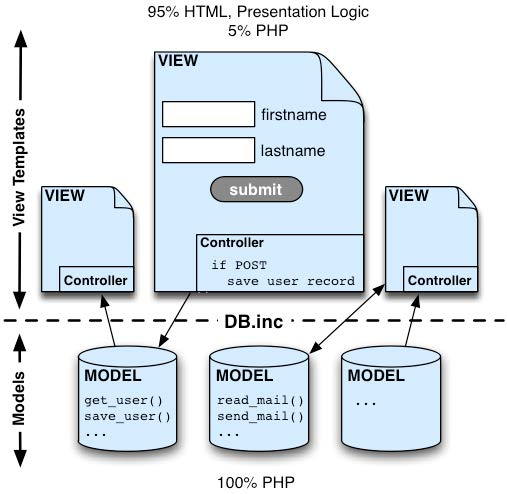
\includegraphics[width=0.5\linewidth]{Images/PHP_MVC.jpg}
		\caption{Example of MVC patter in PHP. Notice that the controller is implemented in a small part of the view templates.}
		\label{fig:php_mvc}
	\end{figure}
	
	Model--View--Controller, usually abbreviated as MVC, partitions a web application into three cooperating responsibilities: the model, the view, and the controller. The pattern is not specific to PHP, but it is particularly relevant in PHP applications because PHP pages can easily combine HTML and executable code in the same file (see figure \ref{fig:php_mvc}). MVC introduces a disciplined boundary between presentation, data manipulation, and request handling.
	
	\subsection{View}
	
	The \textbf{view} is the part of the system where the HTML output is generated and displayed. In PHP this may correspond to a template, a PHP file mainly dedicated to markup generation, or a rendering component provided by a framework.
	
	A view should focus on presentation. It may receive data prepared by the controller or read-only data structures derived from the model, but it should not contain the core business logic of the application. This keeps the generated page easier to inspect and reduces the risk of duplicating application rules across multiple pages.
	
	A minimal PHP-oriented separation can be sketched as follows:
	
	\begin{lstlisting}
	// controller code prepares data
	$userName = $userModel->findDisplayName($userId);
		
	// view code receives data and renders HTML
	<h1>Welcome, <?= htmlspecialchars($userName) ?></h1>
	\end{lstlisting}
	
	The example does not make the view responsible for retrieving the user from the database. Its role is to render the value it has received. Escaping output remains a presentation-layer concern because it depends on the target representation, in this case HTML.
	
	\subsection{Model}
	
	The \textbf{model} provides access to the data to be viewed, collected, modified, or written. In a PHP web application using PostgreSQL, model code typically encapsulates database access and represents the domain-level entities or services that operate on persistent data.
	
	The model should not be reduced to a single database table wrapper. It may include validation rules that depend on the domain, data access methods, transformations, and operations that must remain independent of the page used to trigger them. For example, the same operation for updating a user profile should be reusable whether the request comes from an HTML form, an API endpoint, or a command-line script.
	
	\subsection{Controller}
	
	The \textbf{controller} handles the data that the user inputs or submits and updates the model accordingly. In a web application, this usually means receiving an HTTP request, reading relevant parameters from superglobals such as \texttt{\$\_GET} or \texttt{\$\_POST}, validating and normalizing the input, invoking model operations, and selecting the view that will generate the response.\\
	
	A controller is therefore a coordination layer. It should not contain large portions of HTML, because that responsibility belongs to the view. It should also avoid implementing low-level data access directly, because that responsibility belongs to the model. Its role is to translate a request into application actions and then into a response.
	
	\subsection{Interaction Among MVC Components}
	
	\begin{figure}[!h]
		\centering
		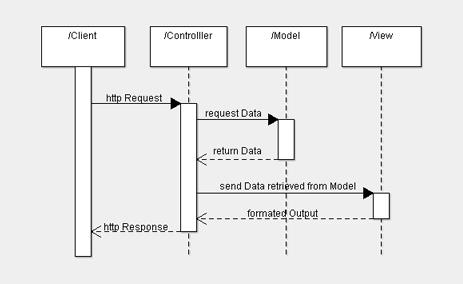
\includegraphics[width=0.5\linewidth]{Images/Request_sequence_diagram.jpg}
		\caption{Sequence diagram of a request handled using the MVC pattern.}
		\label{fig:request_sequence_diagram}
	\end{figure}
	
	All MVC parts are interconnected and share data. This does not mean that every component should access every other component freely. A maintainable PHP application usually keeps the interaction directional and explicit (see figure \ref{fig:request_sequence_diagram}):
	
	\begin{itemize}
		\item the controller receives the request and decides which application operation is required;
		\item the controller invokes model functionality to read or modify data;
		\item the controller provides the view with the data required for rendering;
		\item the view generates the HTML response.
	\end{itemize}
	
	This organization gives a PHP application a clear execution path while preserving the separation of responsibilities. It also makes it easier to test model logic without rendering pages, to change the HTML layout without rewriting data access code, and to reuse common controllers or views across different parts of the site.\\
	
	A typical directory organization may reflect these responsibilities:
	
	\begin{lstlisting}
	project/
	  public/
		index.php
		src/
		  Controller/
			UserController.php
		  Model/
			UserRepository.php
		  templates/
			user-profile.php
	\end{lstlisting}
	
	This structure is only illustrative. Frameworks use different conventions, but the same architectural principle remains: the entry point receives the request, controller code coordinates the application behavior, model code works with data, and templates or views render the response.
	
	\section{PHP Frameworks}
	
	PHP frameworks provide reusable infrastructure for building web applications. They are tools usually based on MVC that help programmers write clearer code in a shorter period of time.\\
	
	A framework typically supplies conventions and components for recurring tasks: routing requests to controllers, rendering templates, managing configuration, integrating database access, handling sessions, organizing validation, and loading application classes. These mechanisms do not replace PHP itself; rather, they structure how PHP code is organized and executed.\\
	
	Frameworks should be understood as libraries and application skeletons, not as extensions automatically built into the PHP engine. Unlike native extensions such as \texttt{pgsql}, framework code is normally loaded as PHP source code, commonly through a Composer autoloader:
	
	\begin{lstlisting}
	require 'vendor/autoload.php';
	use App\Controller\UserController;
	\end{lstlisting}
	
	This distinction matters operationally. A PHP extension becomes available globally after it is installed and enabled in the PHP runtime configuration. A framework or library, instead, is part of the project codebase and must be installed, autoloaded, configured, and deployed together with the application.
	
	\subsection{Symfony}
	
	\begin{figure}[!h]
		\centering
		
\includegraphics[width=0.35\linewidth]{Images/Symfony.jpg}
		\caption{Symfony logo}
		\label{fig:symfony}
	\end{figure}
	
	Symfony is presented as a well-structured and extremely modular framework. Its architecture is extensible and flexible, and its components can be combined to build applications with a clear separation of concerns. Functionality is organized into bundles. In this context, a bundle should be understood as a modular unit that groups related code and configuration. This fits naturally with MVC-oriented development because controllers, views, services, and configuration can be packaged and reused in a structured way.\\
	
	Symfony is therefore appropriate when an application benefits from explicit architecture, modularization, and a rich ecosystem of reusable components. The cost is that the developer must understand the framework conventions and configuration model rather than writing isolated PHP scripts.
	
	\newpage
	\subsection{Zend Framework}
	
	\begin{figure}[!h]
		\centering
		\includegraphics[width=0.35\linewidth]{Images/ZEND_framework.jpg}
		\caption{Zend framework logo}
		\label{fig:zend_framework}
	\end{figure}
	
	Zend Framework is a collection of components. This component-oriented view means that a developer can use parts of the framework to address specific concerns, such as HTTP handling, forms, validation, or database access, instead of relying only on a monolithic application structure.\\
	
	Zend Framework may require a large amount of configuration and coding. This reflects a trade-off common in explicit enterprise-style frameworks: the structure is flexible, but the developer must supply more configuration and integrate the components carefully.
	
	\subsection{CakePHP}
	
	\begin{figure}[!h]
		\centering
		
\includegraphics[width=0.35\linewidth]{Images/Cake_PHP.jpg}
		\caption{Cake PHP logo}
		\label{fig:cake_php}
	\end{figure}
	
	CakePHP is presented as having a strong community and a simple development model based on a limited set of basic rules. Its practical objective is to reduce the amount of application-specific wiring that the developer must write.\\
	
	This style is useful when fast development and predictable conventions are more important than fine-grained architectural configuration. As with any framework, the main benefit appears when the project follows the framework's conventions consistently rather than using it as a loose collection of unrelated utilities.
	
	\section{Choosing Between Plain PHP and a Framework}
	
	The course material does not prescribe a single framework. The relevant design choice is whether the application has reached a level of complexity where framework infrastructure is justified.\\
	
	Plain PHP scripts may be adequate for small pages, prototypes, or narrowly scoped server-side functionality. In such cases, using \texttt{include}, \texttt{require}, functions, classes, and a simple project organization may be sufficient.
	A framework becomes more useful when the application contains several pages, shared layouts, repeated validation rules, persistent sessions, database-backed models, authentication, reusable controllers, and a need for consistent routing and configuration. In these cases, the framework helps enforce an architecture that would otherwise have to be maintained manually.\\
	
	The important point is not that MVC or frameworks add new computational capabilities to PHP. Rather, they organize the capabilities already discussed in the previous chapters into an application structure that is easier to extend, test, and maintain.
	
\end{document}